\documentclass[10pt,a4paper]{article}
\usepackage[margin=18mm]{geometry}
\usepackage[T1]{fontenc}
\usepackage{lmodern,graphicx,booktabs,amsmath,xcolor}
\usepackage[hidelinks]{hyperref}
\setlength{\parindent}{0pt}
\setlength{\parskip}{6pt}
\pagestyle{plain}
\begin{document}
{\Large\bfseries Nontrivial mixed four-kernels in the CM19 model}\par
23 November 2026 \quad Native arithmetic; unsigned [pcc:unverified]

\textbf{Outcome.} The complete fixed-H integral search finds 156 solutions
of $S^\dagger H S=4H$. Of these, 144 have mixed kernel $(4,4,2,2)$;
12 have the multiplication-by-two kernel. The audited primary CM19
bridge connects this model abstractly to the actual smooth F7 quartic.
An explicit coordinate isomorphism and divisor maps remain unconstructed.

\begin{center}
\begin{tabular}{@{}lrl@{}}
\toprule
Integer Smith factors & Count & Interpretation\\
\midrule
$1,1,2,2,4,4$ & 144 & mixed four-kernel\\
$2,2,2,2,2,2$ & 12 & exactly twice a unitary map\\
\bottomrule
\end{tabular}
\end{center}

With $\omega^2=\omega-5$ and $\bar\omega=1-\omega$, the fixed lattice is
\[
 H=\begin{pmatrix}2&1&-1\\1&3&\omega-2\\-1&\bar\omega-2&3\end{pmatrix}.
\]
The first frozen lexicographic mixed matrix is
\[
 S=\begin{pmatrix}
 -4&-2&2\\
 2+2\omega&-1+2\omega&-1-2\omega\\
 -4+2\omega&-3+\omega&3-\omega
 \end{pmatrix}.
\]
Native checks give determinant 8, degree 64, F4 rank 1 and all six Smith
factors above. This map is not divisible by two in the integral endomorphism ring.

\begin{center}
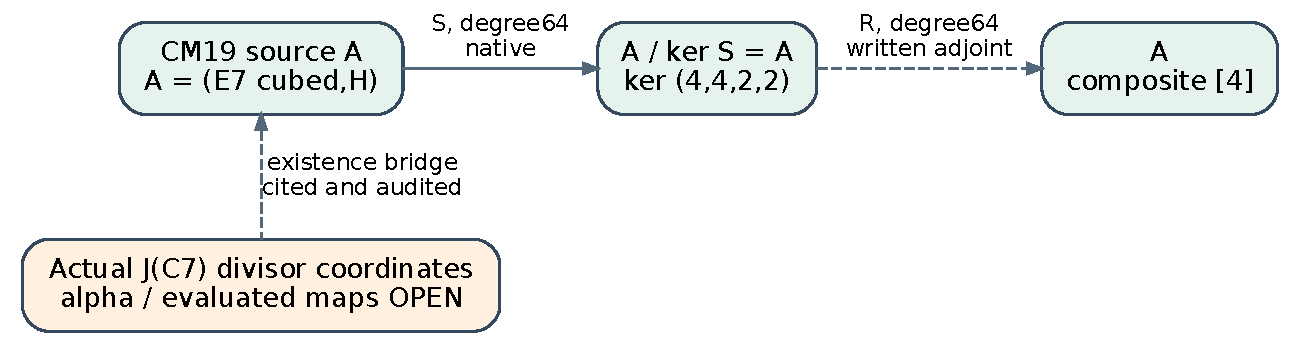
\includegraphics[width=\linewidth,height=51mm,keepaspectratio]{chain.pdf}
\end{center}

\textbf{A written nontrivial chain.}
The integral polarized adjoint $R=H^{-1}S^\dagger H$ satisfies
$RS=4I$ and $R^\dagger HR=4H$. Thus two degree-64 maps factor $[4]$.
R's coefficients and maps have not been separately executed. Each map is
injective on 11-torsion. A rational $(2,2,2)$ first step is excluded by the
even-degree Frobenius composition factors of the source's $J[2]$.
These are mathematical statements with the audited bridge dependencies,
not a completed computational ECDLP reduction or advantage.

Source \texttt{323ece11}; full result \texttt{b2ce1276};
unsigned data \texttt{PCC-20261123-e78d08}. [pcc:unverified]
\newpage
{\Large\bfseries Completeness, actual-source bridge and cost gate}\par

\textbf{A complete fixed-lattice classification.}
H has positive leading minors 2, 5, 1, determinant 1 and inverse diagonal
$(2,5,5)$. Cauchy--Schwarz bounds every coordinate of a vector of norm
at most 12 by O-norm $(24,60,60)$. Since
\[
 N(a+b\omega)=(a+b/2)^2+19b^2/4,
\]
the finite coefficient boxes in the protocol contain every relevant column.
All 252875 grid vectors are checked against the independent six-variable
trace Gram form, whose determinant is $19^3=6859$. No norm-one vector
exists. All 12 unitary maps and all 156 four-similitudes are emitted.

For every four-map, all 923 integer minors determine its Smith factors.
An independent F4 rank agrees; determinant evaluations at both conjugate
roots 3 and 9 modulo 11 are nonzero. The actual $2I$ positive, altered
$(3,2,2)$ diagonal negative and non-Hermitian H mutation controls pass.
Completeness is for this exact H and multiplier four, not all lattices,
polarizations or possible transfers.

\textbf{The genuine-source bridge and its limits.}
The qualified smooth C7 has counts $(17,65,236)$ and Weil polynomial
$(T^2+3T+7)^3$. E7 is ordinary; Frobenius has fundamental discriminant
$-19$, so $\operatorname{End}(E)=\mathbf Z[\pi]=O_{-19}$.
Minkowski's bound is less than three, and two is inert, giving class number
one. Ritzenthaler2010, Propositions3.5/3.6 and Section4.4, supplies the
general equivalence and unique indecomposable Hermitian-class dependencies.
An abstract polarized identification follows using those cited results.
This session audits their hypotheses and H arithmetic; it does not re-prove
the classification or construct the coordinate isomorphism alpha.

\textbf{Computational admission remains held.}
An elliptic input subgroup has $\ell\le p+1+2\sqrt p$, even if the ambient
Jacobian has size about $p^3$. Diem2012, Theorem1, gives a published
$\widetilde O(p)$ plane-quartic DLP bound. Citing that bound alone does
not establish an exponent gain over rho's $O(\sqrt\ell)$ reference.
This compares upper bounds; it is not a lower bound or a measured rejection
of every specialization. These same-field four-maps supply no smaller
prime-field descent. Full strongest-reference conversion, setup, maps,
solve, replay and memory costs still require a separate promising mechanism.

\textbf{Execution and standing.}
All seven strict C phases exit zero; guards unchanged. Rust1.99.1,
warnings denied, overflow/debug assertions, one worker, 2GiB/120s per phase.
All 23 complete locked inputs were read back before execution and all 48
result-commit files afterward. Full stdout is 82374 bytes, SHA256
\texttt{484eca83\ldots ea211ba8}. All 38 small C records are public.
The original 4671000-byte ELF remains temporary custody-pending.
First format, Clippy and pinned reader-prose negatives remain immutable;
display D corrects only its local unsigned marker.

\href{https://github.com/isogeny-labs/crypto/tree/323ece1140a7346630a2f172acc9303e723f3bd0/research/chained_cm19_hermitian_20261123}{Frozen source/protocol/audit}
and
\href{https://github.com/isogeny-labs/crypto/tree/b2ce1276f1b5e967b0bccdb12f1a67e5ee940691/research/chained_cm19_hermitian_20261123}{complete native results}.
Primary sources:
\href{https://doi.org/10.1112/S1461157009000576}{Ritzenthaler (2010)}
and \href{https://doi.org/10.5802/jtnb.815}{Diem (2012)}.
KB/Conductor unavailable; no novelty clearance. Generic Mathlib, actual
divisor/target maps, independent replay, approved custody and normal
paid/vault/experiment/CI/merge requirements persist. [pcc:unverified]
\end{document}
